\section{Stratifying $\RR$}
\label{section:smooth-decompose}

Let $f:M\to\RR$ be a smooth map possessing the stratification conditions of Section \ref{section:smooth-projection} and let $X_f = f(S(f))$, the set of singular values of $f$.
$X_f$ is a connected collection of arcs in the plane that intersect only transversely.

We fit closed neighbourhoods (\emph{sleeves}) around the singular values of $f$ and classify these sleeves by the maximum codimension (with respect to $\RR$) of singular values they contain.
Because $X_f$ consists of codimension 1 and codimension 2 singular values (i.e.\ arcs and arc-crossings respectively), we stratify $\RR$ into face regions that contain no singular values, edge regions that contain only codimension 1 singular values, and vertex regions, each of which contain exactly 1 codimension 2 singular value.
Figures \ref{fig:vertex-sleeve}-\ref{fig:face-sleeve} are used to illustrate the stratification resulting from sleeve-fitting.

\begin{figure}[h!]
	\centering
	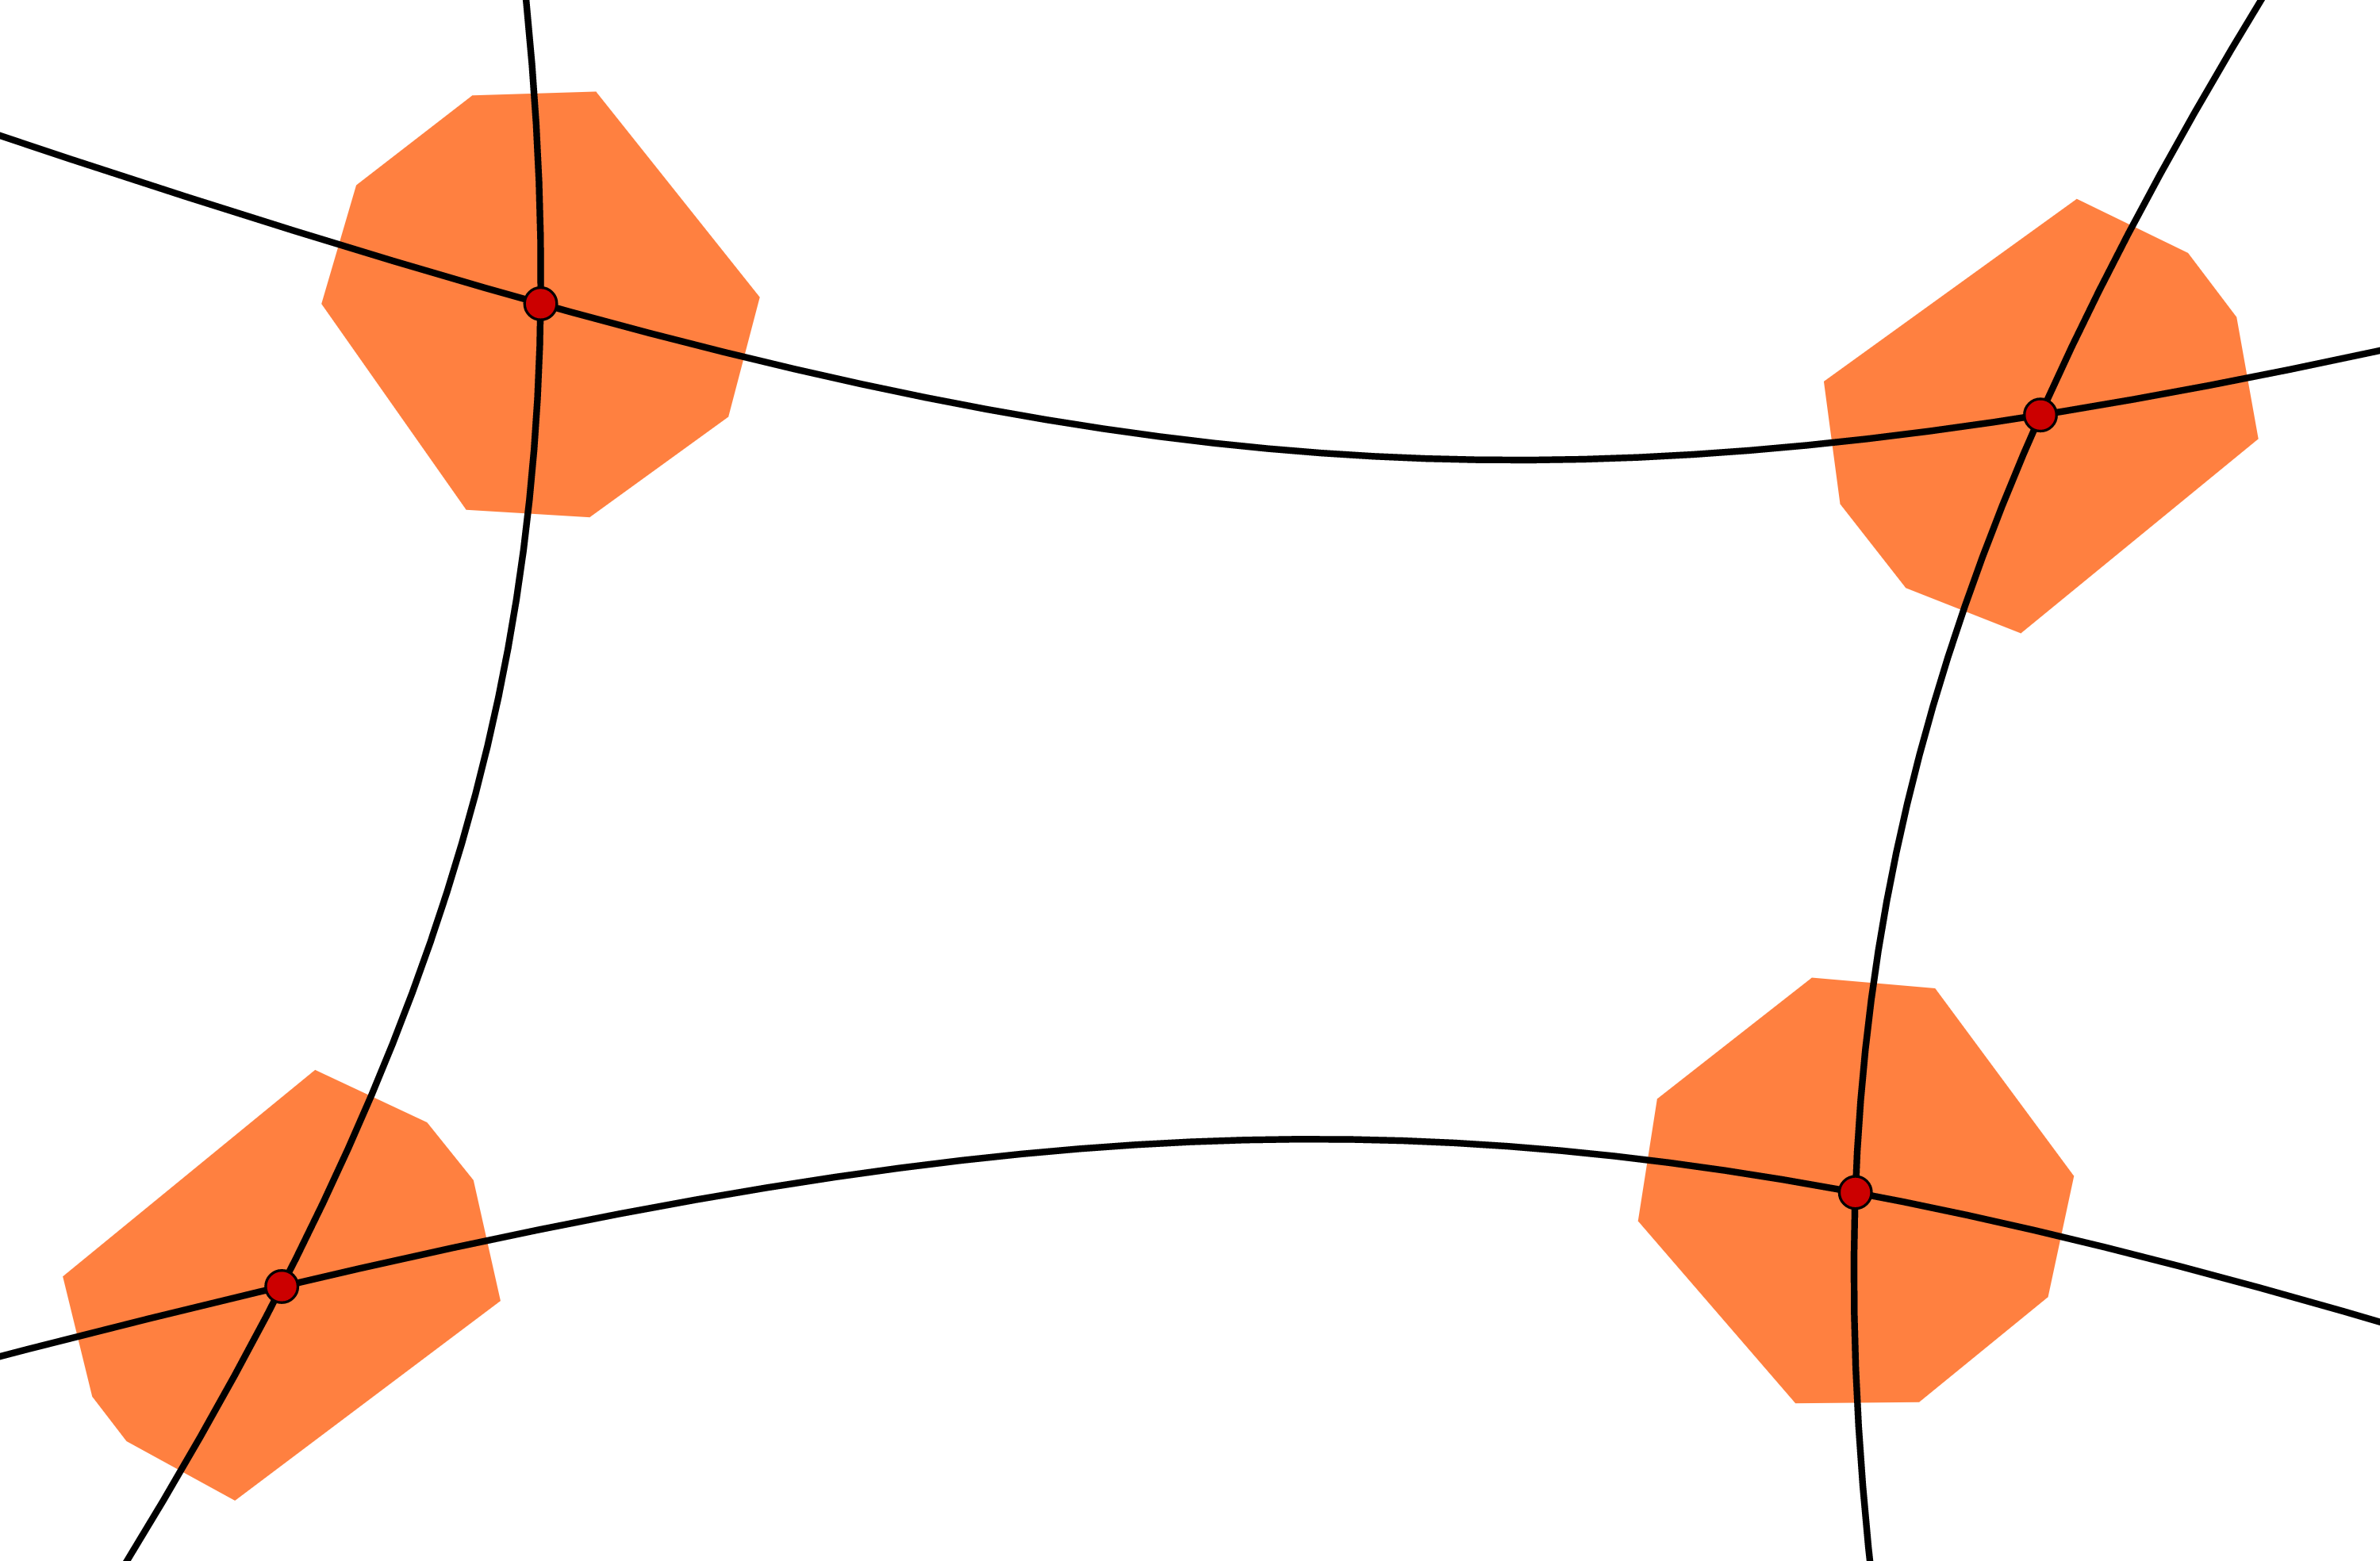
\includegraphics[width=0.5\textwidth]{figures/vertex-sleeve.png}
	\caption{
		\textbf{Forming vertex regions.}
		Octagonal sleeves are fit around codimension 2 singular values to form vertex regions.
		Codimension 1 singular values are illustrated in black and their crossings, codimension 2 singular values, are indicated in red.
		Note that the edges of the octagonal sleeves alternate between containing exactly one singular value, its intersection with a black arc, or consisting entirely of regular values.
	}
	\label{fig:vertex-sleeve}
\end{figure}

We begin by fitting octagonal sleeves around codimension 2 singular values as in Figure \ref{fig:vertex-sleeve}.
%Octagons are used here solely to simplify descriptions further down the line of proof.
Let $x$ be a codimension 2 singular value.
$x$ is the result of an arc crossing, and a small neighbourhood around an arc crossing is divided into four regions of regular values.
The octagon around $x$ is fit so its edges alternate between being fully contained in a region of regular values and orthogonally intersecting one of the arcs of singular values that creates $x$.
See Figure \ref{fig:vertex-sleeve} for a model fitting.

The interiors of the octagons along with the octagonal boundaries form the vertex regions of the stratification of $\RR$.
The octagons are chosen to be small enough that no two vertex regions overlap and such that the octagonal edges that intersect arcs of codimension 1 singular values are all the same length.

\begin{figure}[h!]
	\centering
	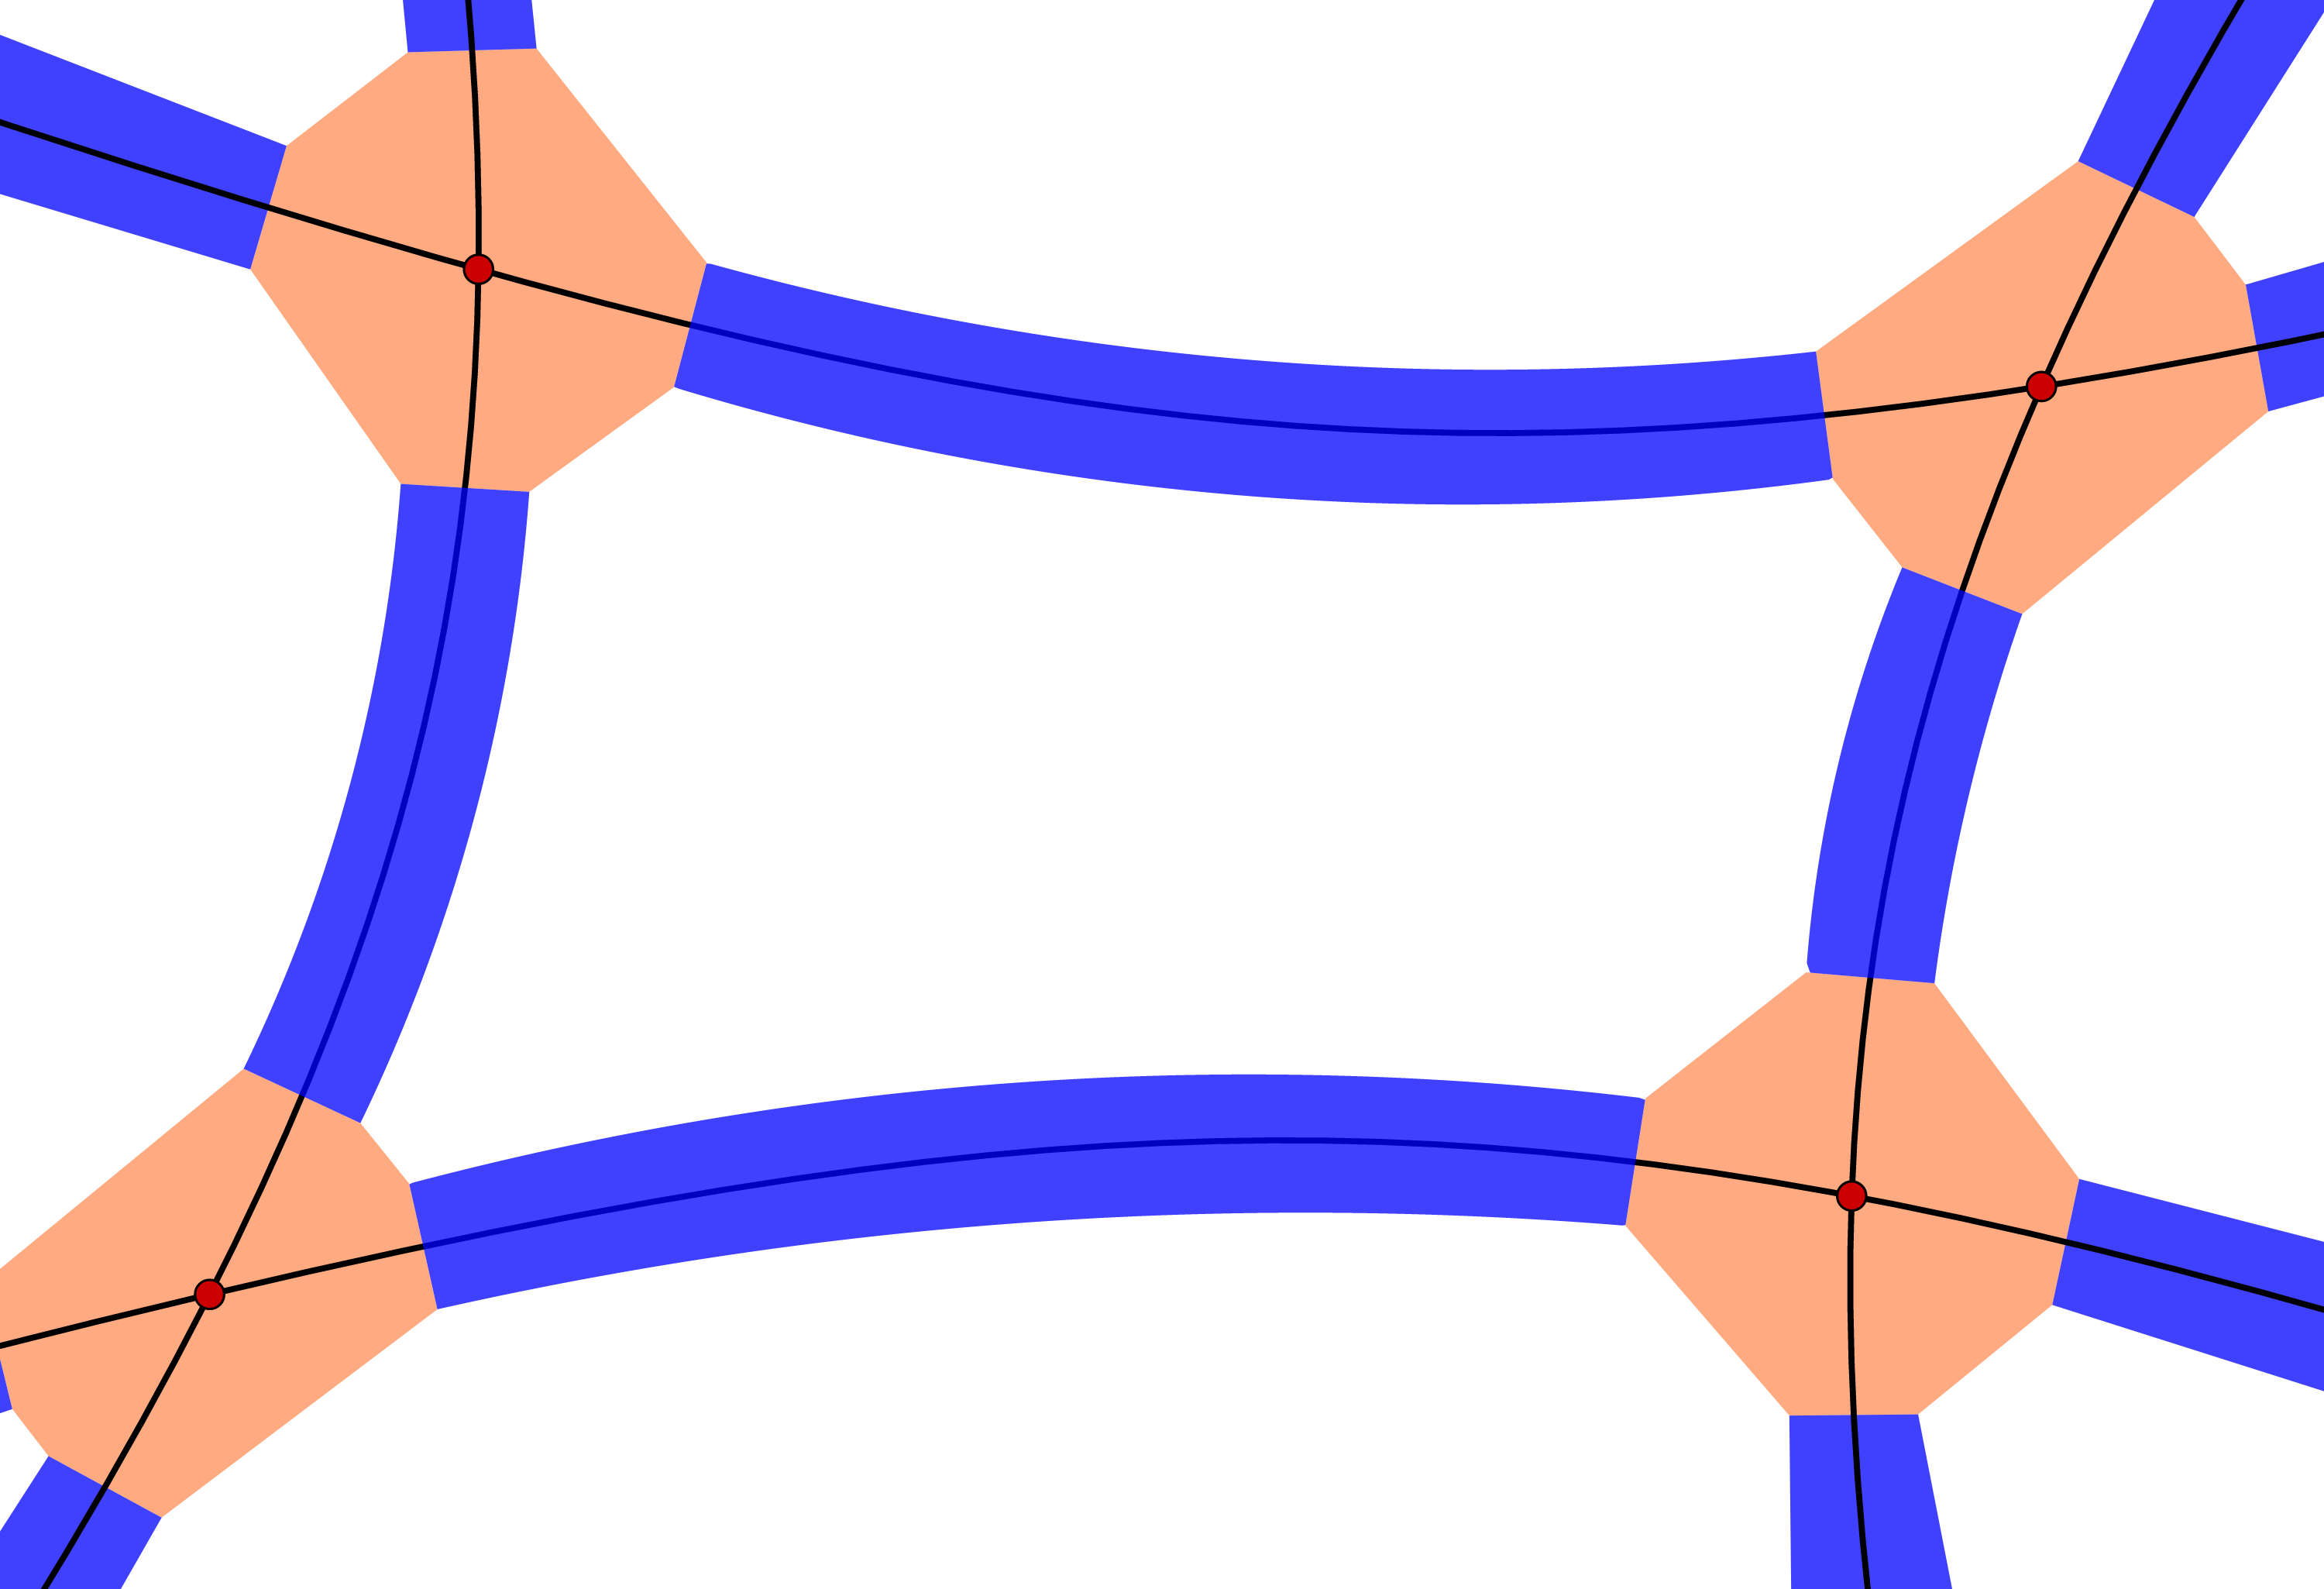
\includegraphics[width=\textwidth]{figures/edge-sleeve.png}
	\caption{
		\textbf{Forming edge regions.}
		Vertex region corners are connected to fit sleeves around arcs of codimension 1 singular values to form edge regions.  
	}
	\label{fig:edge-sleeve}
\end{figure}

Let $\gamma$ be an arc of codimension 1 singular values with endpoints a pair of codimension 2 singular values.
$\gamma$ orthogonally intersects one edge from each of the octagonal vertex regions fit around its endpoints, and we use these edges to form the edge region associated to $\gamma$ by connecting the endpoints of these edges to one another using a pair of arcs parallel to $\gamma$.
See Figure \ref{fig:edge-sleeve} for a model fitting.

The closures of the interiors of the shapes formed by the arcs and octagon edges form the edge regions of the stratification of $\RR$.
The octagonal edge endpoints are also vertices of the octagons, and the formation of edge regions uses every octagonal vertex as the endpoint of exactly one arc.

\begin{figure}[h!]
	\centering
	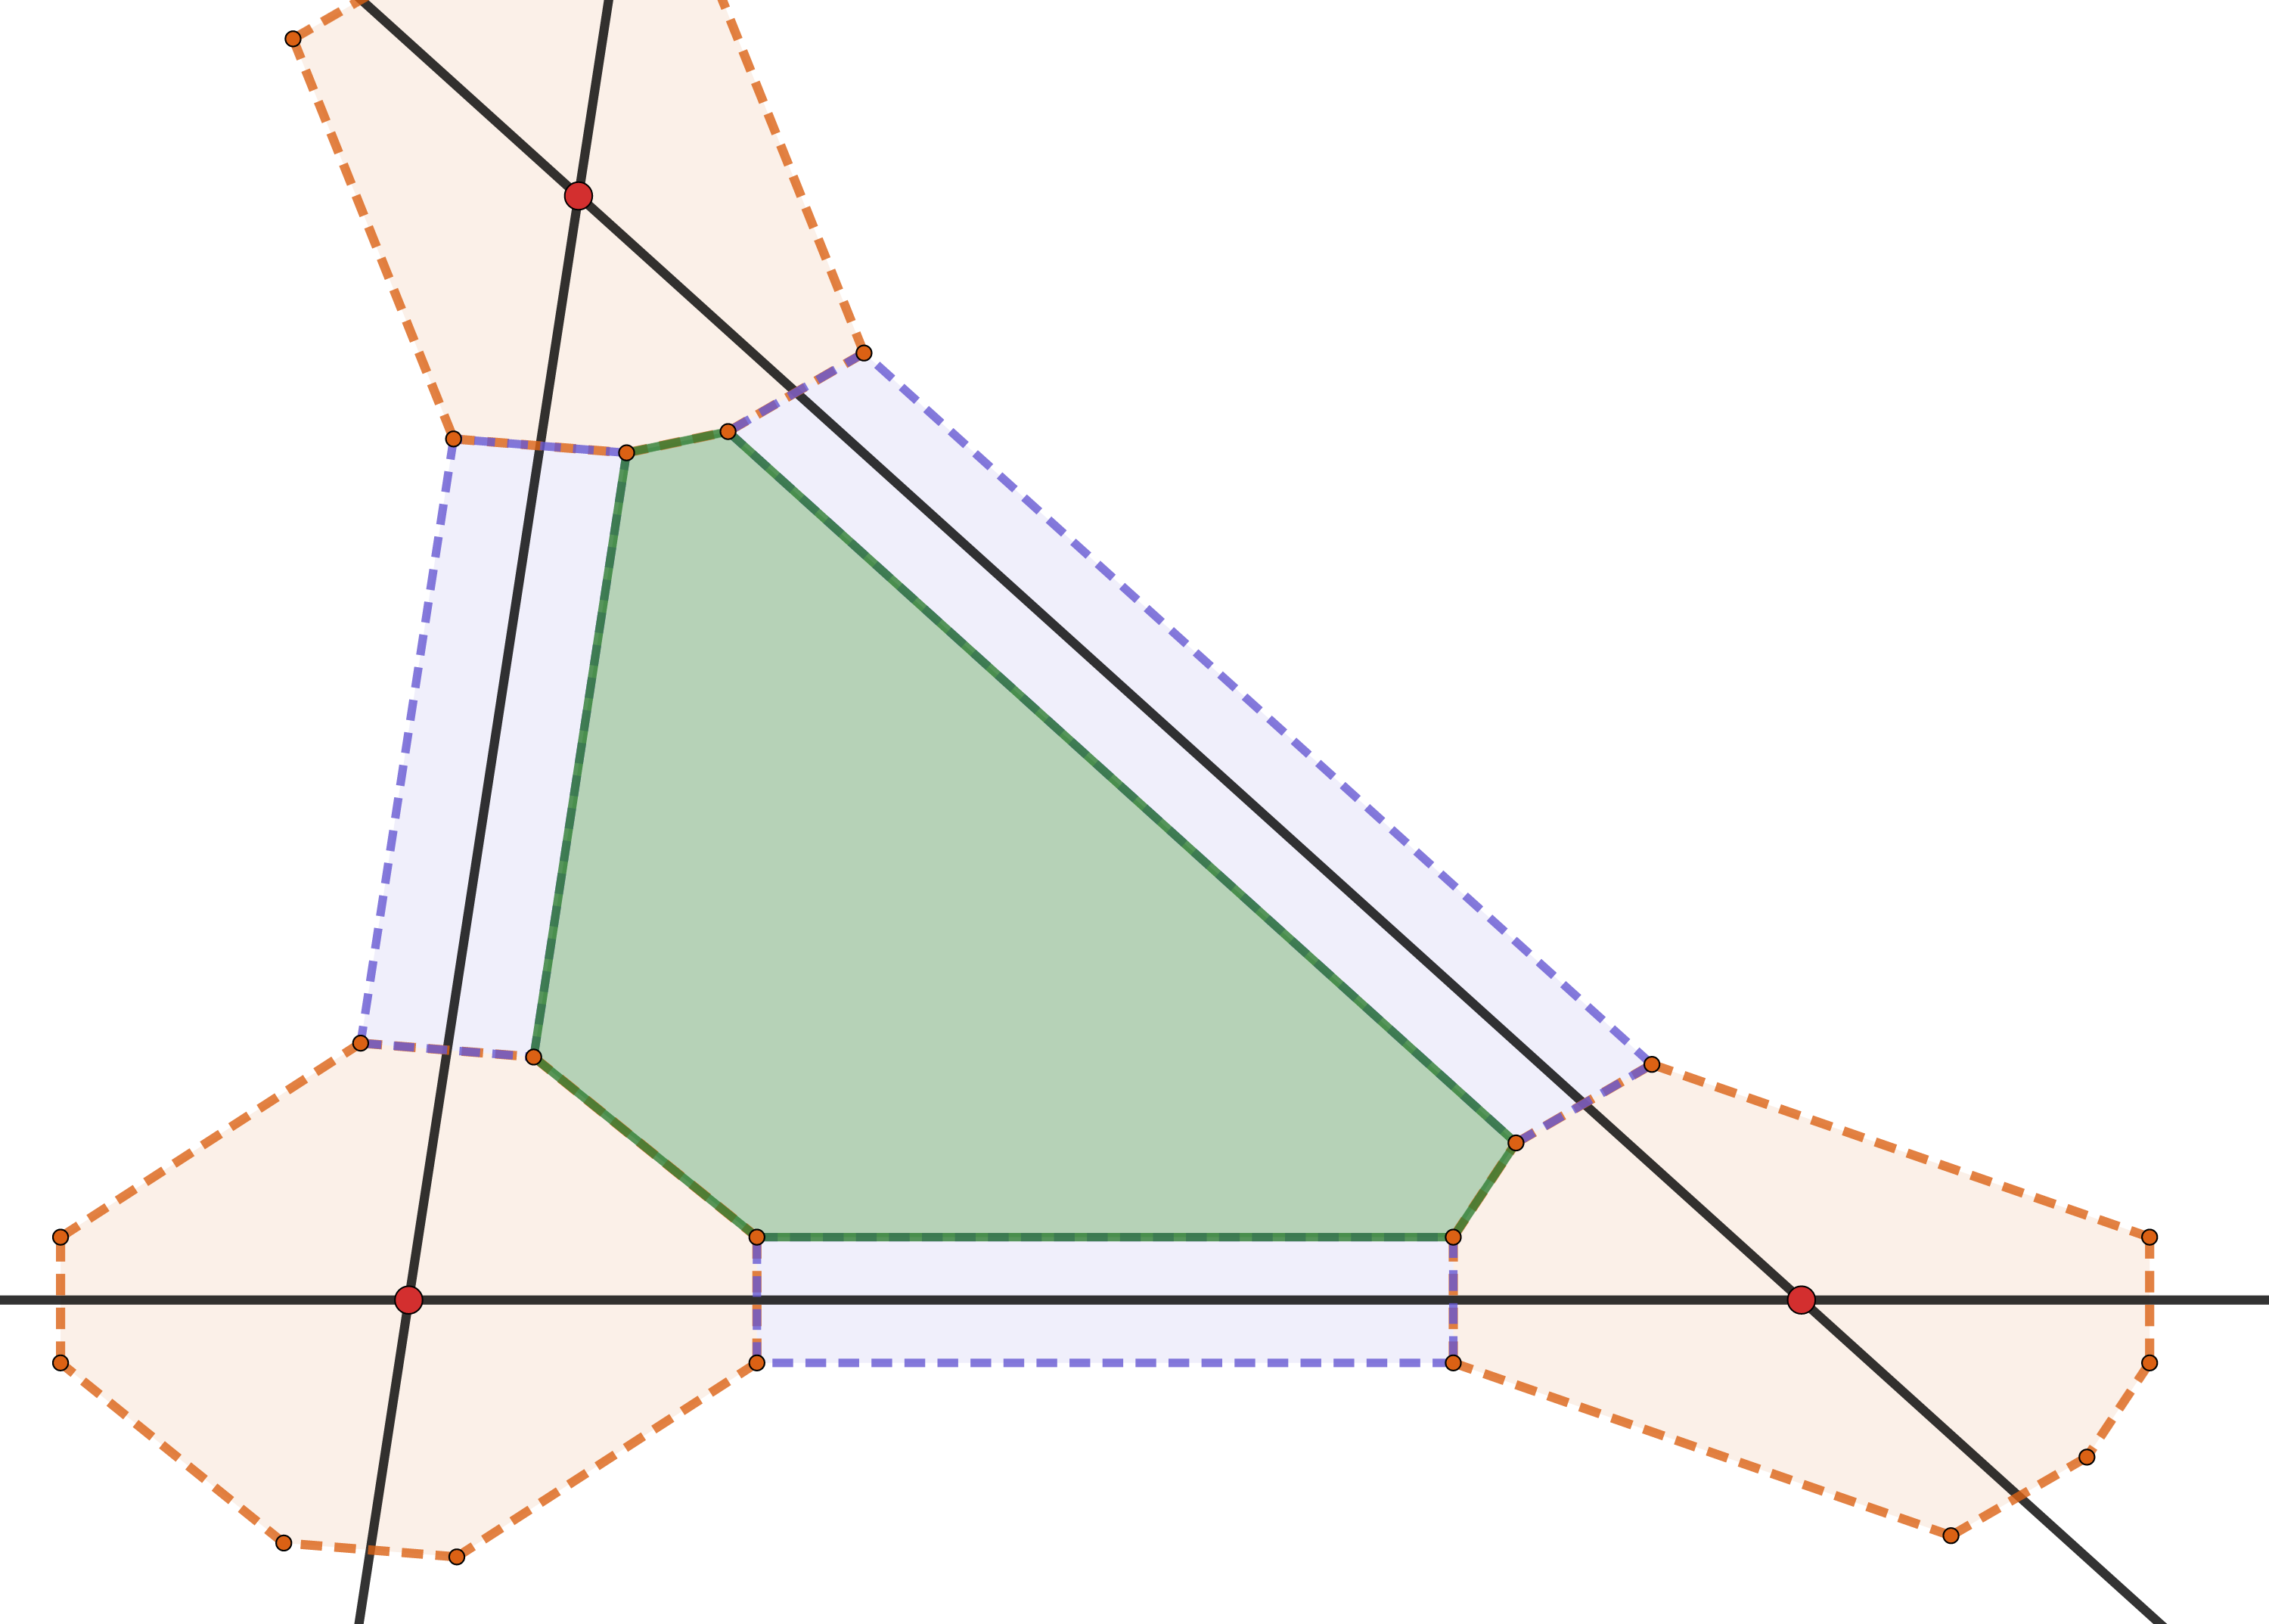
\includegraphics[width=\textwidth]{figures/face-sleeve.png}
	\caption{
		\textbf{Forming face regions.}
		All remaining regions contain no singular values, and we take these to be the face regions.
	}
	\label{fig:face-sleeve}
\end{figure}

Removing from $f(M)$ all vertex and edge regions, we are left with a collection of simply connected regions in the plane, each of which consists entirely of regular values.
We take the closures of these to be the face regions of the stratification of $\RR$.
The boundary of each face region is an alternating collection of arcs from edge regions and octagonal edges from vertex regions.
See Figure \ref{fig:face-sleeve} for a model fitting.

With all of the regions defined, we can describe precisely how $f$ stratifies $\RR$.
The stratification of $\RR$ is a stratification into subsets $R_{(i,j)}$ where $i,j$ are integers.
Subset indexing is defined so that a subset $R_{(i,j)}$ is an $i$--dimensional submanifold of $\RR$, thus $R_{(i,j)}\nleq R_{(k,l)}$ if $i\nleq k$.
The first collection of subsets used to filter $\RR$ are the corners of the octagonal vertex sleeves.
We assign to these subsets the indices $(0,i)$ for $i=1\dots N_0$, where $N_0$ is the number of corners.
Corners are disjoint, hence $R_{(0,i)}$ is not contained in $R_{(0,j)}$ for any $i, j$, whence $(0,i)\nleq (0,j)$ for any $i,j$.

The boundary arcs connect the $(0,i)$--level strata.
Arcs are indexed by $(1,j)$ for $j=1\dots N_1$, where $N_1$ is the number of arcs.
The boundary points of an arc are corners and are subsets of the filtration indexed by the $(0,i)$ indices, so $(0,i)\leq (1,j)$ if and only if $R_{(0,i)}$ is one of the boundary points of $R_{(1,j)}$.
Arcs intersect only at their boundary points, so $(1,j)\nleq(1,k)$ for any $j,k$. 

The regions themselves are indexed by $(2,k)$ for $k=1\dots N_2$, where $N_2$ is the number of regions.
These indices work similarly to the arc indices.
The boundary of a region consists of corners and arcs, so $(n,i)\leq(2,k)$ if and only if $R_{(n,i)}$ is contained in the boundary of $R_{(2,k)}$.

With $\RR$ stratified, we move onto a stratification of $M$.
This stratification is induced by the preimages of the strata of $\RR$.

%
%Before moving on to the stratification of $M$ induced by our decomposition of $\RR$, we need to iron out the corner cases of when $X_f$ contains no codimension 2 singular values.
%
%
%Because $X_f$ is connected, $X_f=f(S_1(f))$, and $S_1(f)$ is a collection of smooth non-intersecting curves in $M$, we conclude that $S_1(f)$ contains exactly one curve.
%Furthermore, $f(M\setminus S_1(f))$ lies entirely within $X_f$ so $S_1(f)$ is everywhere a definite fold.
%
%...

